\subsection{Simulation and Simplified Model}
The previous sections show a velocity model of the system which is modelled in this section. As mentioned in the inertia test, \appref{app:inertiaTest}, the armature inductance is so small that it is not necessary to include for a good simulation. If the armature inductance is neglectable, and removed, the system will appear as a first order system instead of a second order. Therefore \si{L_a} is set to zero and hence removing the second order term. This effect is illustrated in the transfer function:
%
\begin{flalign}
  \eq{\frac{V(s)}{U_a(s)}}{ \frac{K_t}{L_a \cdot J_{tot} \cdot s^2 + (R_a \cdot J_{tot} + L_a \cdot B_{tot}) \cdot s + R_a \cdot B_{tot} + K_t \cdot K_e }}\nonumber\\
  &\Downarrow&\nonumber\\
  \eq{\frac{V(s)}{U_a(s)}}{ \frac{ K_t }{ R_a \cdot J_{tot}  \cdot s + R_a \cdot B_{tot} + K_t \cdot K_e }}\nonumber\\
  \eq{\frac{V(s)}{U_a(s)}}{ \frac{ \frac{K_t}{R_a \cdot B_{tot} + K_t\cdot K_e} }{ \frac{R_a \cdot J_{tot}}{R_a \cdot B_{tot} + K_t \cdot K_e}\cdot s + 1 }}
  \label{eq:simplifiedTransferVel}
\end{flalign}
%
By inspection of the first order expression, in \eqref{eq:simplifiedTransferVel}, the terms for the time constant and the gain are extracted:
\begin{flalign}
  \eq{K}{\frac{K_t}{R_a \cdot B_{tot} + K_t\cdot K_e}}&\nonumber\\
  \eq{\tau }{ \frac{R_a \cdot J}{R_a \cdot B_{tot} + K_t \cdot K_e} }\nonumber&
\end{flalign}
%
To verify that this is a viable approximation, the following simplified model, in \figref{fig:BlockDiagramDrivetrainSimplified}, is created:
%
\begin{figure}[H]
	\centering
	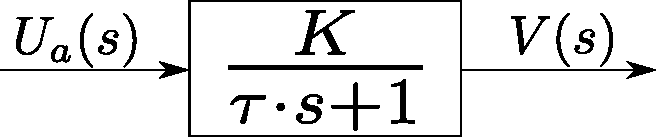
\includegraphics[scale = .5]{figures/totalVelocityModelDiagramSimplified.pdf}
	\caption{A block diagram showing a simplified model}
	\label{fig:BlockDiagramDrivetrainSimplified}
\end{figure}
%
Where \si{K} is the gain of the system and \si{\tau} is the time constant. This simplified first order model of the system is simulated alongside the second order model, to verify that the vehicle can indeed be handled as a first order system. The plot of the two simulations are illustrated in \figref{fig:ComparisonOf1stAnd2ndOrderModels}.
%
From this figure it is impossible to see any difference between the two models, however, zooming in on the base of the step, see \figref{fig:comparison1stAnd2ndOrderModelsZoom}, the difference becomes clear.
%
\begin{minipage}{\linewidth}
  	\centering
  	\begin{minipage}{0.45\linewidth}
  		\begin{figure}[H]
  			\centering
  			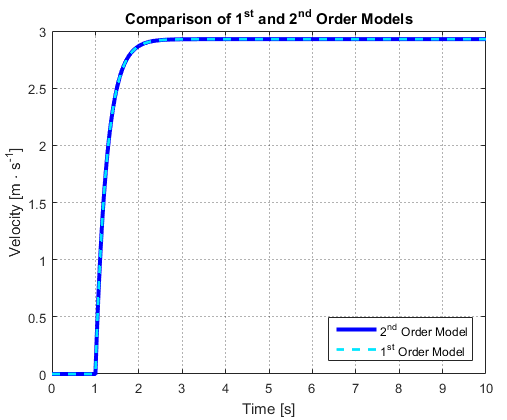
\includegraphics[scale = .6]{figures/ComparisonOf1stAnd2ndOrderModels.png}
  			\caption{Comparison of the \si{1^{st}} and \si{2^{nd}} order models}
  			\label{fig:ComparisonOf1stAnd2ndOrderModels}
  		\end{figure}
  	\end{minipage}
  	\hspace{0.03\linewidth}
  	\begin{minipage}{0.45\linewidth}
  	  \begin{figure}[H]
    	 	\centering
    	 	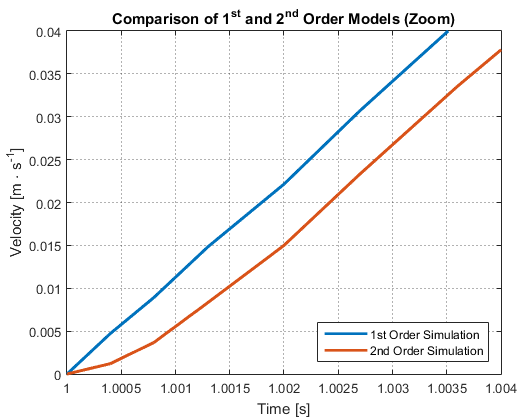
\includegraphics[scale = .6]{figures/comparison1stAnd2ndOrderModelsZoom.png}
    	 	\caption{Comparison of the \si{1^{st}} and \si{2^{nd}} order models}
    	 	\label{fig:comparison1stAnd2ndOrderModelsZoom}
    	\end{figure}
  	\end{minipage}
  \end{minipage}

However, a quick glance at the axes shows how minimal the impact of this difference must be. An other and possibly clearer way to show the difference of the two models, is through use of Bode plots. A Bode plot of the two models imposed on one another is seen on \figref{fig:bodePlotOf1stAnd2ndOrderModel}.
%
\begin{figure}[H]
	\centering
	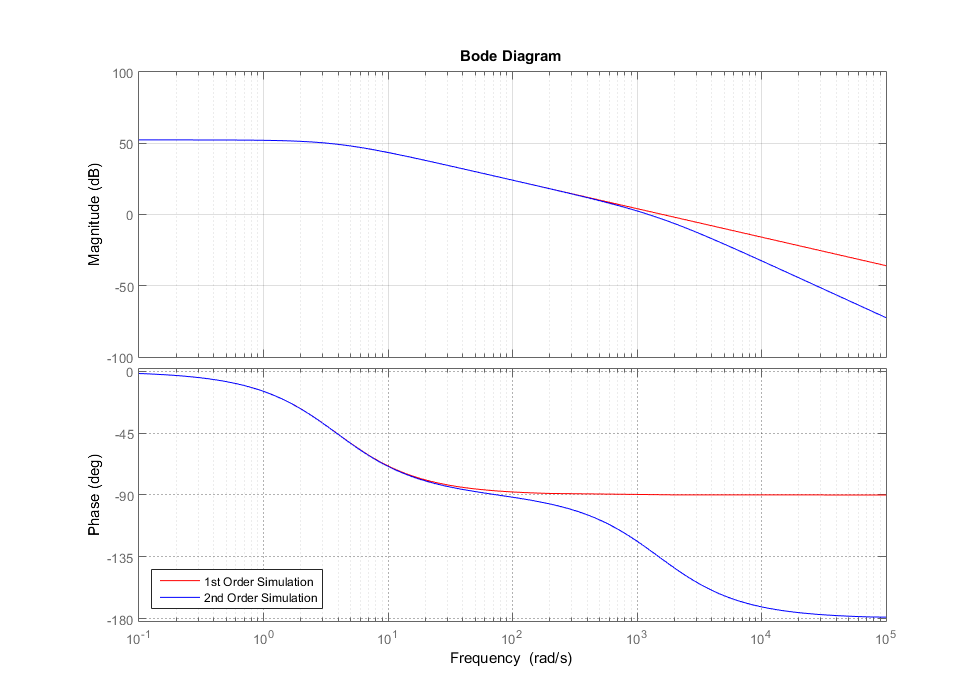
\includegraphics[width = \textwidth]{figures/bodePlotOf1stAnd2ndOrderModel.png}
	\caption{Bode plot showing the differences between the \si{1^{st}} and \si{2^{nd}} order models}
	\label{fig:bodePlotOf1stAnd2ndOrderModel}
\end{figure}
%
For frequencies below 1000 \si{rad\cdot s^{-1}} the two models are very similar because each of their first poles are very close; in 3,8759 \si{rad\cdot s^{-1}} for the \si{1^{st}} order model and 3,9 \si{rad\cdot s^{-1}} for the \si{2^{nd}} order model. The \si{2^{nd}} order model however has an other pole which causes the phase shift and shift in magnitude at higher frequencies. However since this pole is so high, 1489,5 \si{rad\cdot s^{-1}}, it does not affect the lower pole considerably and the differences are way beyond significant frequency range.

In the following section the simplified model is verified directly by comparison with recorded data of the vehicle's step response.